% small.tex
\RequirePackage{atbegshi}

\documentclass{beamer}
\usetheme[height=7mm]{Rochester}

\usepackage{graphicx}
\usepackage{hyperref}
\usepackage{skull}
\usepackage{verbatim}
\usepackage[utf8]{inputenc} 
\usepackage[T1]{fontenc}
\usepackage[czech,english]{babel}


\title{Autíčko + webkamera + neuronová síť + = awesomesauce}
\author{Michal Demín, Kuba Marek}
\date{}

\begin{document}

\begin{frame}[plain]
\titlepage
\end{frame}

\begin{frame}{Základní myšlenka}
\begin{itemize}
\item Motion vectors -- odhad pohybu v obrazu, používá se v MPEG
\item Detekce kolizí:
Když vidím nějaký objekt jako statický, pak jsem na kolizním kurzu.
\end{itemize}
\end{frame}

\begin{frame}{Přehled}
\begin{itemize}
\item
\end{itemize}
\end{frame}

\hspace{-1.39cm}
\begin{frame}[plain]
\begin{centering}
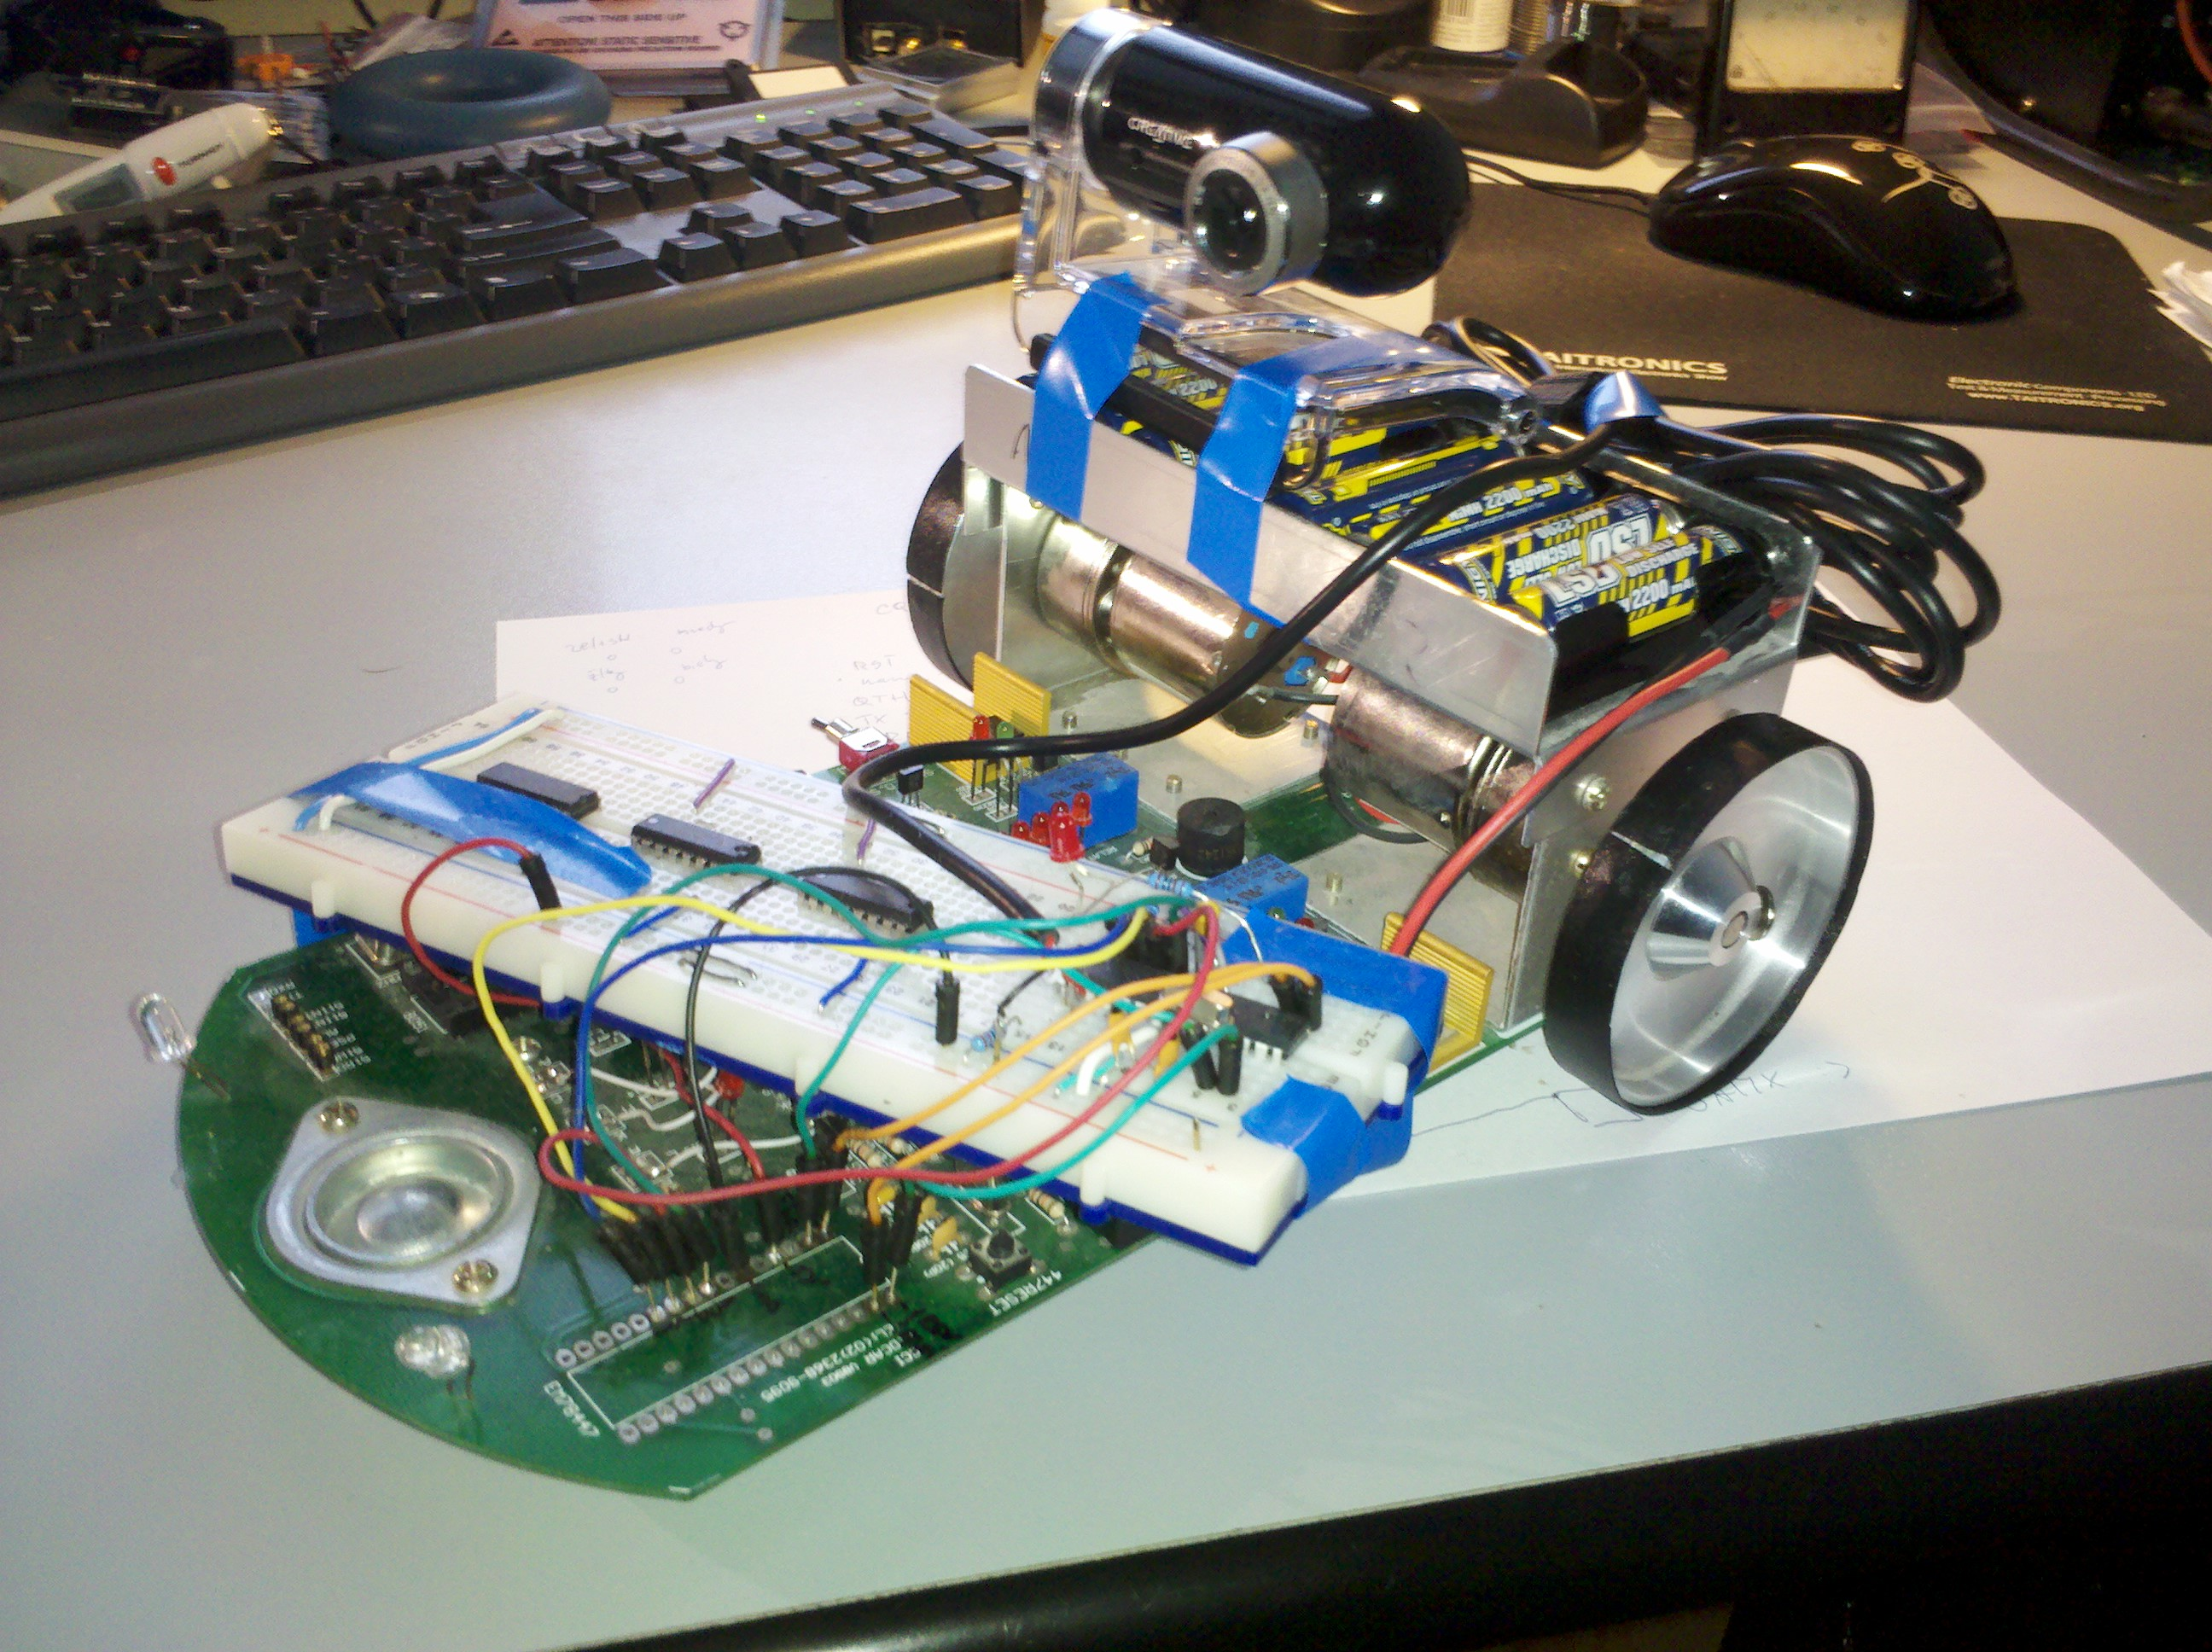
\includegraphics[width=1.05\paperwidth]{img1.jpg}
%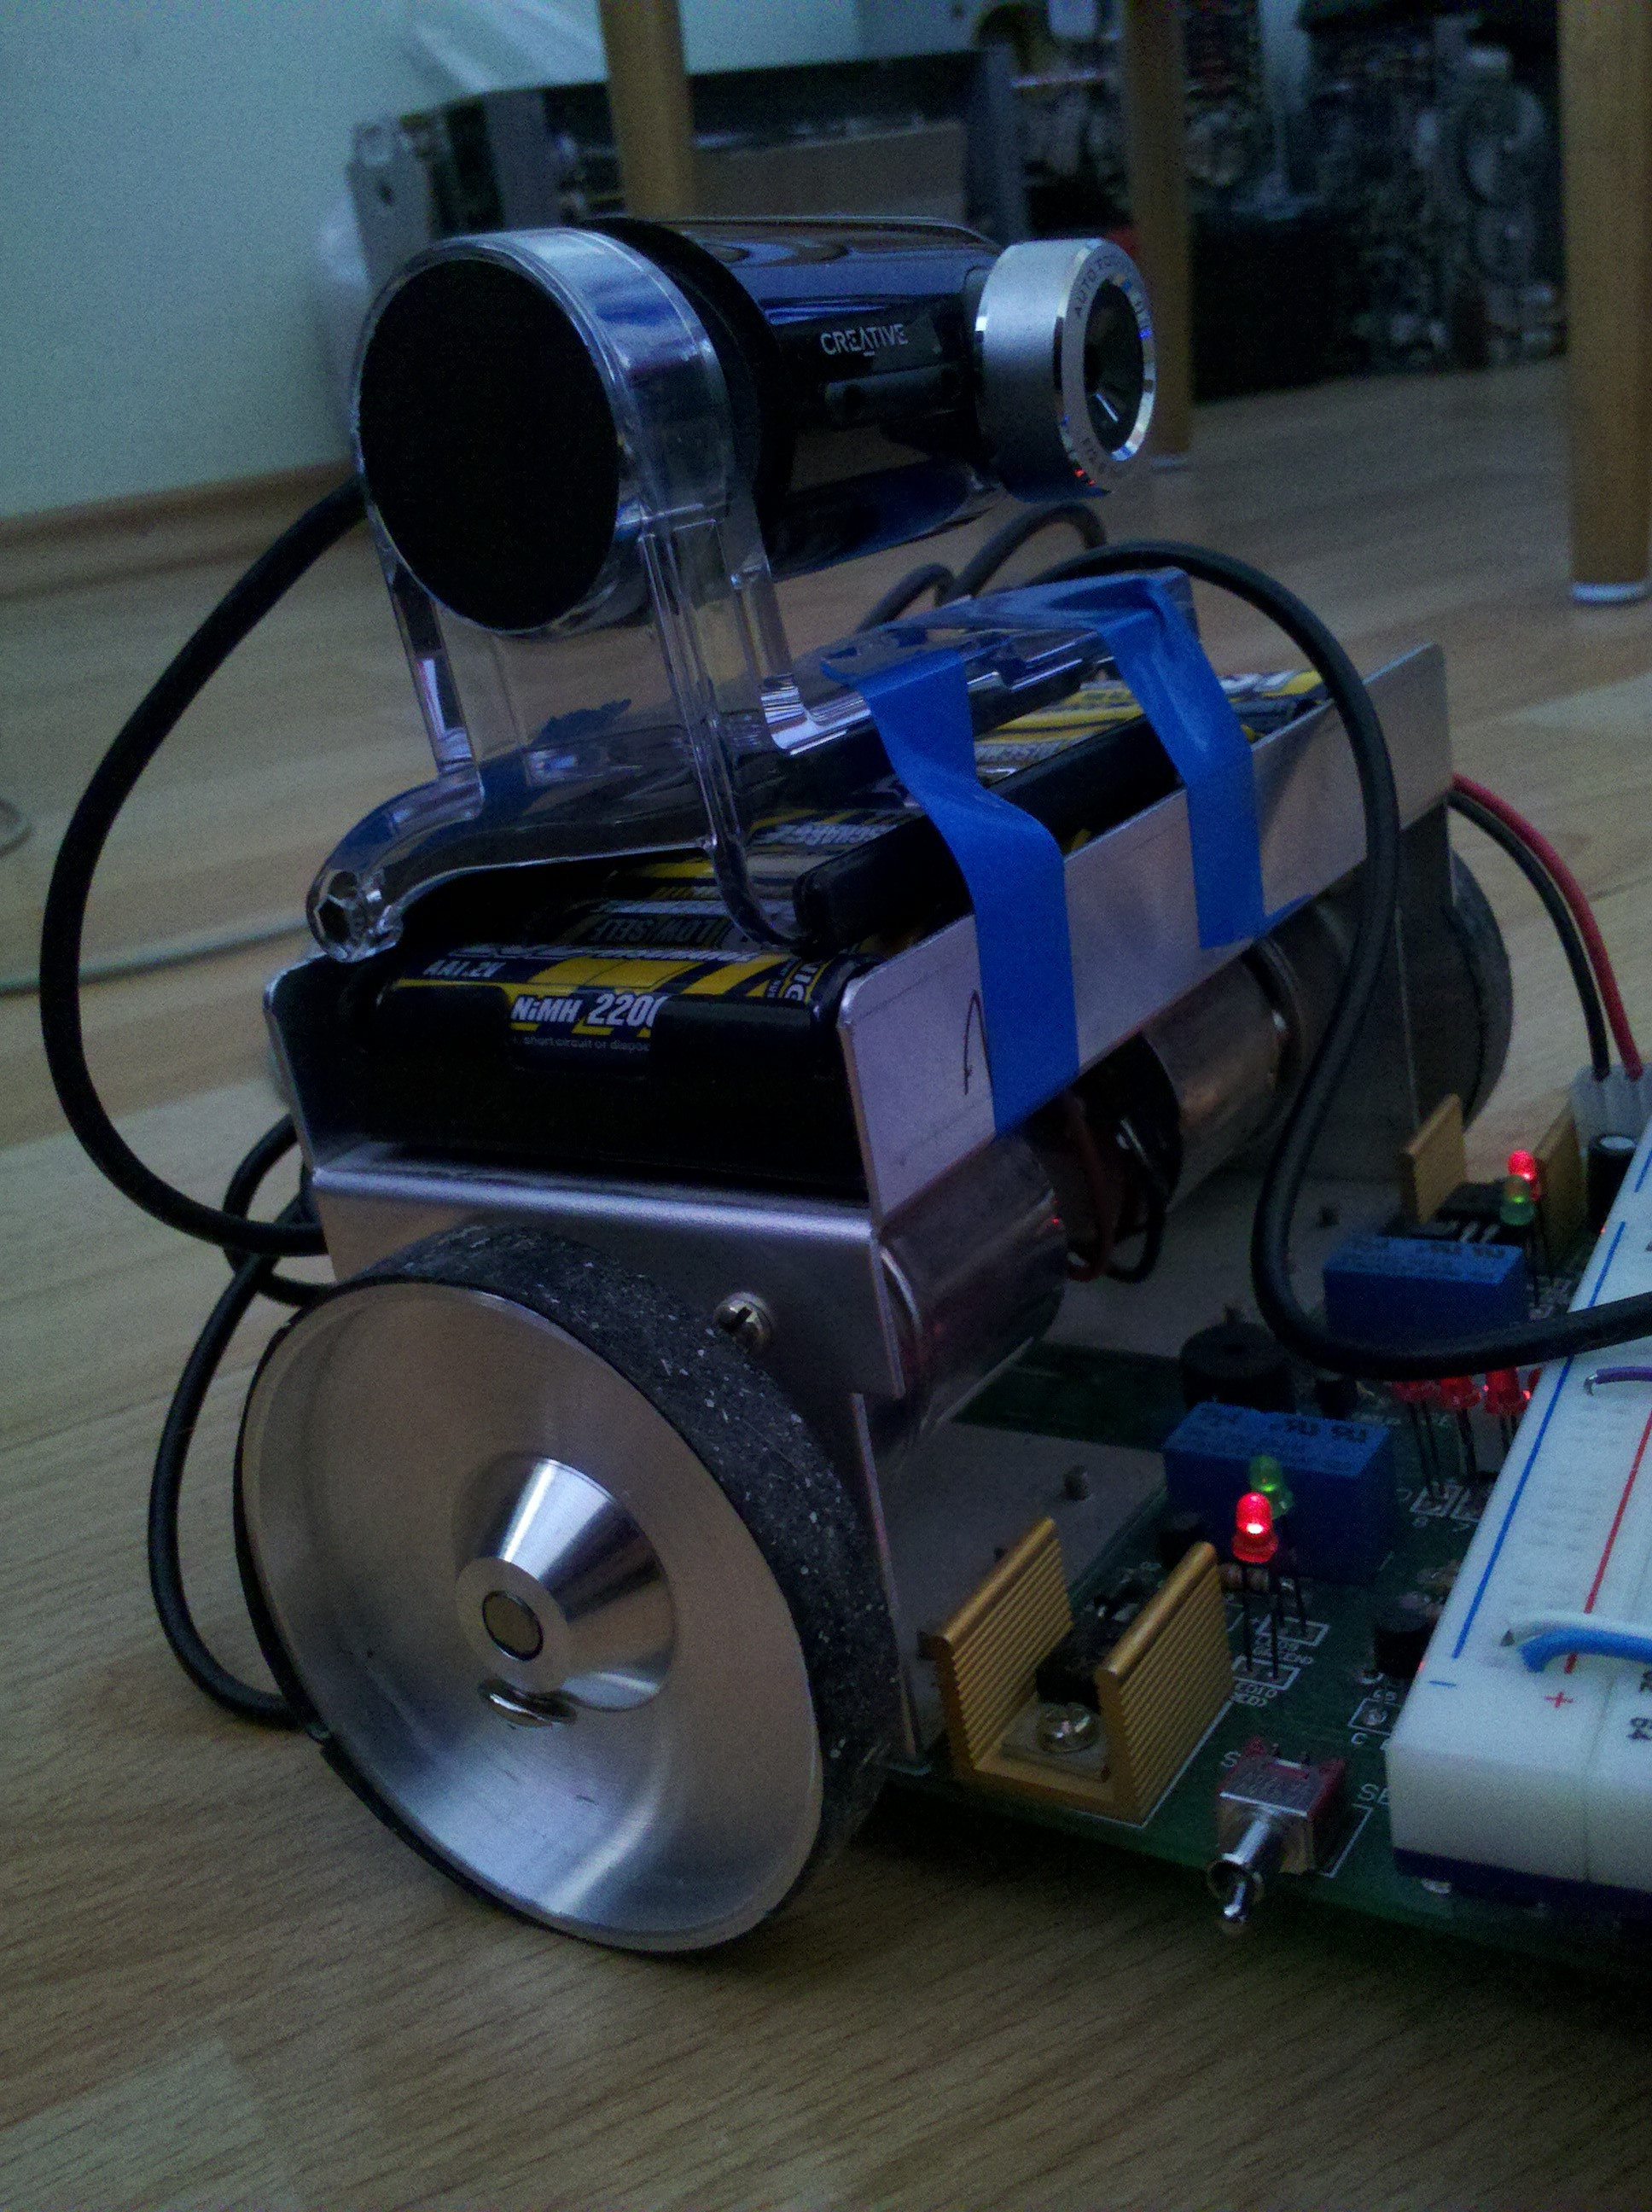
\includegraphics[height=0.5\textheight]{img2.jpg}
\end{centering}
\end{frame}

\begin{frame}{Co funguje}
\end{frame}

\begin{frame}[plain]
\center
Video!
\end{frame}

\begin{frame}{Preprocessing}
\begin{itemize}
\item
\end{itemize}
\end{frame}

\begin{frame}{Neuronová síť}
\begin{itemize}
\item
\end{itemize}
\end{frame}

\begin{frame}{Problémy}
\begin{itemize}
\item Webkamera
	\begin{itemize}
	\item Pouze MJPEG, nebo raw bitmapy -- Řešení: OpenCV
	\item Zpoždění obrazu
	\item Nevhodný zorný úhel
	\item Automatické ostření
	\end{itemize}
\item Podvozek
	\begin{itemize}
	\item Podkluz -- Řešení: Pogumování koleček
	\item Nepřesné řízení a velká setrvačnost
	\end{itemize}
\end{itemize}
\end{frame}


\end{document}
